%%%%%%%%%%%%%%%%%%%%%%%%%%%%%%%%%%%%%%%%%
% This template has been downloaded from:
% http://www.LaTeXTemplates.com
% Original author:
% Frits Wenneker (http://www.howtotex.com)
% License:
% CC BY-NC-SA 3.0 (http://creativecommons.org/licenses/by-nc-sa/3.0/)
%%%%%%%%%%%%%%%%%%%%%%%%%%%%%%%%%%%%%%%%%

\documentclass[11pt,a4paper]{scrartcl} 
\usepackage[english]{babel}
\usepackage{amsmath,amsfonts,amsthm} % Math packages
\usepackage{lipsum} % Used for inserting dummy 'Lorem ipsum' text 
\usepackage{sectsty} % Allows customizing section commands
\usepackage{booktabs}
\usepackage{multirow}
\allsectionsfont{\centering \normalfont\scshape} 
\usepackage[toc,page]{appendix}
\usepackage[parfill]{parskip}
\usepackage{graphicx}
\usepackage{subcaption}
\makeatletter
\setlength{\@fptop}{0pt}
\setlength{\@fpbot}{0pt plus 1fil}
\makeatother

%----------------------------------------------------------------------------------------
%	TITLE SECTION
%----------------------------------------------------------------------------------------

\newcommand{\horrule}[1]{\rule{\linewidth}{#1}} % Create horizontal rule command with 1 argument of height

\title{	
\normalfont \normalsize 
\textsc{Loyola Marymount University, Department of Computer Science} \\ [25pt] 
\horrule{0.5pt} \\[0.4cm]
\huge Assignment 0925 \\ 
\horrule{2pt} \\[0.5cm]}

\author{Joaquin Loustau\\}
\date{\normalsize\today} 
\begin{document}
\maketitle
\begin{abstract}
The term wearable technology refers to electronic technologies or computers that are incorporated into items of clothing and accessories which can comfortably be worn on the body. Examples of wearable devices include \textit{Google Glass}, a device with an optical head-mounted display and smartwatches \textit{Moto 360} and \textit{The Pebble}. This report analyzes the performance of these devices for specific tasks in terms of three usability metrics (learnability, errors and satisfaction) both quantitatively and qualitatively.
\end{abstract}

%----------------------------------------------------------------------------------------
% USABILITY METRICS
%----------------------------------------------------------------------------------------

\section{Usability Metrics}
The results of the tests performed on the wearable devices \textit{The Pebble}, \textit{Moto 360} and \textit{Google Glass} indicated \textit{The Pebble} as being overwhelmingly superior in terms of usability. \textit{The Pebble}, a smartwatch developed by Pebble Technology Corporation and released in 2013, ranked 1st in all three categories: lowest average time to perform a task, lowest number of errors and greatest average satisfaction (see Appendices).\\
\hspace*{\fill} \\
The tasks assigned were the following:
\begin{enumerate}
	\item Send a specified message (``Hi, how are you?") to a specified contact (Steve Smith). 
	\item Set a timer for one (1) minute.
	\item Check the weather for today at the current location. The task concludes when the test subject is able to give the high temperature for the day.
\end{enumerate}
\hspace*{\fill} \\
These were the usability metrics measured:
\begin{enumerate}
	\item Time to learn (\textit{learnability}).
	\item Rate of errors by users (\textit{errors}).
	\item Subjective satisfaction (\textit{satisfaction}) on a scale from 1-10, with 10 being the highest and 1 being the lowest.
\end{enumerate}
\textit{Google Glass} performed the worst out of the three systems tested in average time to complete tasks, with an average time of 50 seconds, and in satisfaction, with an average satisfaction of 6.09 out of 10. \textit{Moto 360} had an average of 3.72 errors per task per user, a satisfaction of 7.45 out of 10 and an average time to complete a task of 45 seconds.
%----------------------------------------------------------------------------------------
% HEURISTIC EVALUATION
%----------------------------------------------------------------------------------------

\section{Heuristic Evaluation}
The following subsections will explore possible reasons \textit{why} the assigned systems (\textit{Google Glass}, \textit{Moto 360} and \textit{The Pebble}) performed the way they did in the tasks previously described. The discussion will be based on interaction design principles, theories, interaction styles, and guidelines documents of the assigned devices.

\subsection{Google Glass}
Sending a message to a specified number, checking the high temperature for today and setting a timer for one minute all seem simple, concrete and straightforward tasks.\textit{Google Glass}, as described by its Design Principles, ``works best with information that is simple, relevant and current."\cite{google01}  Nevertheless, \textit{Google Glass} was the system analyzed that performed considerably the worst all factors considered. When test subjects used \textit{Glass} to perform the assigned tasks, it took them the longest time to complete the task, had several errors and felt the lowest satisfaction with their experience in comparison with the other two systems.

Prior to delving into the reasons why \textit{Glass} performed the way it did, it is necessary to make some clarifications. Firstly, it is important to note that test subjects got significantly more frustrated at \textit{Glass} than at \textit{The Pebble} and \textit{Moto 360} when the system did not behave as expected. The main reason for this appears to be that \textit{Google Glass} is so close to the user's senses that unexpected functionality and bad experiences generate high levels of frustration and anger in a short span of time. \textit{Google Glass'} screen does not interfere with the field of vision, so the user is not exclusively focused on the screen but also on what is happening in his surroundings. As the user notices motions in his surroundings, his head and eyes deviate, and the ongoing process in \textit{Glass} is affected, thus generating exasperation.

Along these lines, \textit{Google Glass} presents an unfamiliar hardware to most test subjects. On the other hand, although the majority of the individuals performing the tasks had not operated a smartwatch before, they were all familiar with the shape of the hardware (alike an ordinary watch), and the gestures involved in operating it. In fact, \textit{The Pebble} looks no different than a digital watch to most people who first encounter it. The unfamiliarity of \textit{Google Glass'} hardware should certainly be accounted for when analyzing the results.

When setting up the timer in \textit{Google Glass}, most test subjects had no problem selecting the option from the main menu by using the voice command ``start a timer." However, the users that did not immediately see the option in the main menu had problems to launch the timer screen, as they tried using the voice command "set a timer," which is not a valid command. This situation is a clear example of the series of complex and diverse factors that are involved in making design interaction decisions. \textit{Google Glass} developers express in their Voice Command Guidelines that voice commands should ``bring the user from intent to action as quickly as possible and not sound similar to existing commands."\cite{google02} By selecting the command ``start a timer" rather than ``set a timer," developers avoided the possibility of getting the voice command confused with ``set an alarm" during voice recognition. However, this decision came at the sacrifice of consistency in the interaction style employed. While natural language is used all throughout the system, command language was used for this one command, ``start a timer".

Once the test subject was able to activate the voice command for the timer, he/she was directed to a new screen with a timer set to zero (0) hours, zero (0) minutes and zero (0) seconds (similar to  Figure 1). The vast majority of users said ``one minute" expecting it to be a valid voice command to set up the timer. However, the timer cannot be set up and started by voice command from this screen but must be set up using the touch pad on the side of \textit{Google Glass} - first sliding from back to front and then tapping. This was the only error recorded for this task for most test subjects and responds to a lack of consistency in data display, one of the high-level objectives Smith and Mossier offer as part of their guidelines for data entry, and one of the Eight Golden Rules of interface design.\cite{plaisant09} Users had to use the voice command first, then swipe and finally tap the touch pad to eventually start the timer. This same problem was observed with \textit{Moto 360}, as it will be later discussed.

\begin{figure}[h]
\centering
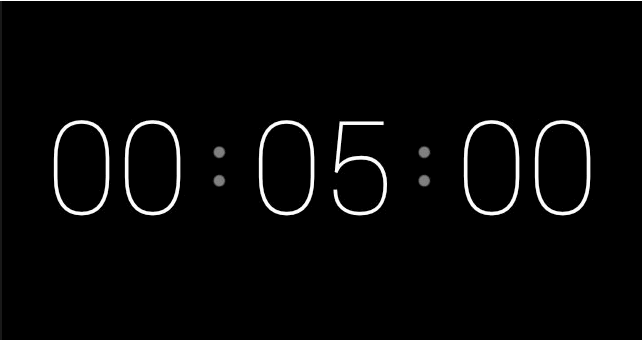
\includegraphics[width=3 in]{glass_timer.png}
\caption{\textit{Google Glass'} timer lacks consistency in data input}
\end{figure}


In contrast to the timer task, \textit{Google Glass} performed relatively well when sending a text message to a specific contact. Its sound performance can be explained by the fact that \textit{Google Glass} exploits (mostly) natural language commands and keeps a minimal amount of input actions by the user -except in the cases already discussed. By having the user launch the message application with the voice command ``send a message to [name of the recipient]" the user solely needs to include the body of the message (see Figure 2). The content of the message is input via voice command as the screen prompts the question ``What is the message?” No more commands are required after the screen prompt and the message is immediately sent.

\begin{figure}[h]
\centering
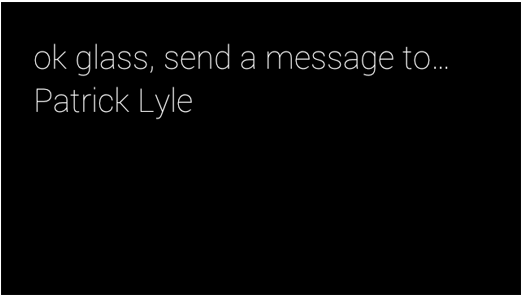
\includegraphics[width=3in]{glass_message.png}
\caption{Message interface for Google Glass.}
\end{figure}

The task that involved finding the highest temperature for the day at the current location had mixed performances. The users who were able to accomplish the task in a short time were the ones who did not hesitate to access Google search through the \textit{Glass} menu. A card with the current weather, including high and low temperature appeared and the task was completed. 

One of the main reasons some test subjects had difficulties in completing this task was \textit{Google Glass'} inconsistent visibility. This component of an interaction design is strictly connected with the psychology of causality, for when ``an action has no apparent result, you may conclude that the action was ineffective. So you repeat it. It is a poor design that allows either kind of false causality to occur."\cite{norman02} After users asked Google for the weather (by saying Ok \textit{Glass}, Google...), \textit{Glass} sometimes displayed a ``loading" screen and other times just displayed an empty black screen (see Figure 3). Users were confused by this, and unsure whether they needed to use another voice command. A few test subjects were in the process of restarting the task when \textit{Glass} unexpectedly displayed the weather information. The lack of or inconsistent feedback was the main reason for \textit{Glass'} poor performances for this task. \textit{Google Glass} failed to keep its users informed about ongoing processes and  provide clear error messages. 

\begin{figure}[h]
\centering
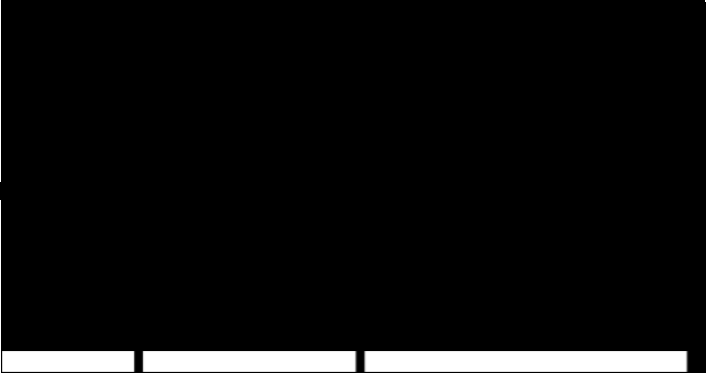
\includegraphics[width=3in]{glass_loading.png}
\caption{The loading screen is not always displayed.}
\end{figure}

As an experienced user, I can also attest \textit{Google Glass'} failure to support internal locus of control. In spite of having owned and used a pair of \textit{Google Glass} for several months, I do not often have the sense that I am in charge of the interface or that the interface responds to my actions.  
The following extract from \textit{The Design of Everyday Things} seems to perfectly encapsulate the reasons for \textit{Google Glass'} performance, as well as to shed some light on its future, \textit{``It usually takes five or six attempts to get a product right. This may be acceptable in an established product, but consider what it means in a new one. Suppose a company wants to make a product that will perhaps make a real difference. The problem is that if the product is truly revolutionary, it is unlikely that anyone will quite know how to design it right the first time; it will take several tries. But if a product is introduced into the marketplace and fails, well that is it. Perhaps it could be introduced a second time, or maybe even a third time, but after that it is dead: everyone believes it to be a failure."}
\cite{norman02}

\subsection{Moto 360}
\textit{Moto 360} performed extremely well in sending a message and setting a timer, but poorly in finding the high temperature for the current day and location. 

The main reason why \textit{Moto 360} performed so poorly in the task involving checking the weather was its reliance on command language. This made it extremely hard for novice users to access the information requested, as the command needed to access the weather did not match logical, explicit, everyday phrases. The only voice commands \textit{Moto 360} seemed to recognize were ``weather," ``weather in Los Angeles" and ``weather current location.” All other commands, such as ``what is the weather like?", ``what is the highest temperature for today?" or ``weather forecast" were considered invalid by \textit{Moto 360}, triggering a Google search rather than retrieving the weather information. Once the Google search was launched, the user had to give full attention to the device to try to find an answer through the search engine or find the option to go back, therefore contradicting three core design principles of Android wear: ``focus on not stopping the user and all else will follow," ``do one thing, really fast" and ``design for the corner of the eye."\cite{moto360}

Furthermore, and only if the user was in fact able to activate the weather voice command, a card displaying the current temperature and atmospheric conditions popped up (see Figure 4). To access the highest and lowest temperatures for the day, it was necessary to swipe from right to left to obtain more information from the card. This proved to be a counter intuitive movement for most test subjects, who tried tapping the weather card instead.

\begin{figure}[h]
\centering
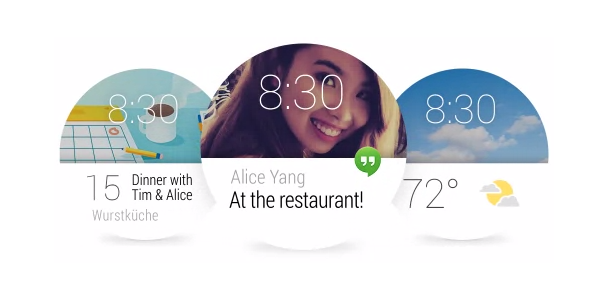
\includegraphics[width=3in]{moto_cards.png}
\caption{Most users found it difficult to realize they had to swipe the weather card(right) to see the highest and lowest temperatures.}
\end{figure}

The \textit{Moto 360} menu is inconsistent with the principle ``Design for big gestures"\cite{moto360} found in the Design Principles for Android wear, as it does not use few and large touch targets, but rather an extensive list of small icons and verbose commands, such as:
\begin{itemize}
	\item \textbf{take a note} drink more water
	\item \textbf{remind me} to go for a run at 7am
	\item \textbf{show me my steps}
	\item \textbf{show me my heart rate}
	\item \textbf{send a text to} Jim, you around?
	\item \textbf{email} Eve, you free on Friday?
	\item \textbf{agenda} for today
	\item \textbf{navigate} to a gas station nearby
	\item \textbf{set a timer} for 30 minuets
	\item \textbf{start stopwatch}
	\item \textbf{set an alarm} for 3 hours from now
	\item \textbf{show alarms}
	\item \textbf{settings}
\end{itemize}

Given the complexity of the voice commands offered in the Google Now menu, many test subjects decided to just scroll down the screen to find the specific tasks in the menu list. It took them a few seconds to find the options ``send a text" and  ``set at timer", which appears to contradict the already mentioned principle, ``to design for the corner of the eye." This principle expresses that ``the longer the user is looking at your app, the more you are pulling them out of the real world"\cite{moto360} and therefore interactions between the user and the watch should be simple and brief.
 
\subsection{Pebble}
\textit{The Pebble's} outstanding performance seems to support the aphorism ``less is more," often attributed to German-American architect Ludwig Mies van der Rohe. Although \textit{Pebble's} graphic interface is far from being as aesthetic as \textit{Glass'} or \textit{Moto 360's} interfaces, \textit{Pebble's} simplicity seems to be the main reason why this device was so well received by novice users.

\textit{The Pebble} maximizes Scheidernman's ``Golden Rules" and Nielsen's Ten Usability Heuristics. \cite{plaisant09} There are only four (4) possible inputs that can be selected, using the buttons on either side of the watch: back, up, down, and select -these commands respond to \textit{The Pebble's} Menu Selection interaction style (see Figure 5). The user feels in control of the system at all times (internal locus of control) and there is no sequence of commands he needs to memorize (minimal user memory load). The lack of voice command operations prevents errors by standardizing the input and reducing the range of different input actions by users. However, the lack of a dial/crown or other mechanism to scroll down the menu options without having to press the down button several times implies a higher number of button clicks to complete the desired task. Sending the message involved 12 button clicks, setting the timer 8, and checking the weather 10. As a side note, a possible solution to this might be to redesign the hardware so that the select button is a crown that can be both rotated and pressed.

\begin{figure}[h]
\centering
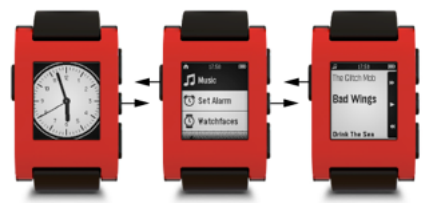
\includegraphics[width=3in]{pebble_buttons.png}
\caption{Pebble users navigate by means of button clicks, windows and menu items.}
\end{figure}

On the other hand, it is foreseeable that the limited options of \textit{The Pebble} might eventually not be enough for users with more expertise. Besides the possibility of installing new apps, it does not seem as increased proficiency enables increased functionality -``beyond this basic functionality the beauty of \textit{Pebble} is that people can expand the power and capability of their smartwatch by choosing to acquire, download, and install a host of \textit{Pebble} apps."\cite{pebble01}  In this sense, \textit{The Pebble} fails to accommodate multiple user profiles. Since the metrics measured were learnability, errors and satisfaction, the results do not reflect feedback from expert users. 

When observing \textit{The Pebble's} Design Principles and comparing them side by side with the experience test subjects had using the device, one finds a direct correlation.\textit{The Pebble} does ``focus on the simplest way for the user to interact with a complex data" and ``keeps the pattern of engagement with the user consistent and intuitive" (see Figure 6). This explains its exceptional performance. 

\begin{figure}[!t]
\centering
\begin{subfigure}{.5\textwidth}
  \centering
  \caption{}
  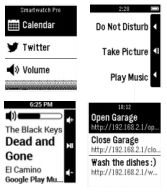
\includegraphics[height=.52\linewidth]{pebble_screens.png}
\end{subfigure}%
\begin{subfigure}{.5\textwidth}
  \centering
  \caption{}
  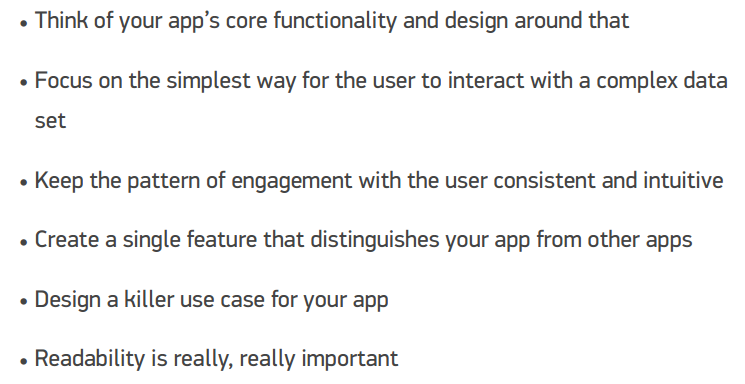
\includegraphics[width=1\linewidth]{pebble_designprinciples}
\end{subfigure}
\caption{Pebble screens compared side by side with Pebble's Design Principles}
\end{figure}

\clearpage
\begin{thebibliography}{9}
\bibitem{google01}
 Google Glass Design Principles. 
https://developers.google.com/glass/design/principles

\bibitem{google02}
 Google Glass Voice Command Checklist.
 https://developers.google.com/glass/distribute/voice-checklist
 
\bibitem{plaisant09}
Ben Shneiderman and Catherine Plaisant.   \emph{Designing the User Interface: Strategies for Effective Human-Computer Interaction}
  Addison Wesley/Pearson ,
  5th edition,
  2009.

\bibitem{norman02}
Donald A.Norman \emph{The Design of Everyday Things}
  Basic Books,
  2002.
  
\bibitem{moto360}
Design Principles for Android Wear.
https://developer.android.com/design/wear/principles.html


\bibitem{pebble01}
Developer Guide:Pebble UX Design.
http://assets.getpebble.com.s3-website-us-east-1.amazonaws.com/dev-portal/UX-Design-Guide-v1.1.pdf

\end{thebibliography}
\pagebreak
\begin{appendices}
\begin{table}[h!]
\caption{Send message ``Hi, how are you?" to Steve Smith.} 
\centering
\begin{tabular}{@{}llccc@{}}
\toprule
Person & Device & Time & Errors & Satisfaction \\ \midrule
Infante, Brian & Moto 360 & 1:05 & 5 & 4 \\
 & Google Glass & 0:59 & 2 & 5 \\
 & Pebble & 0:20 & 0 & 9 \\
Fitzpatrick, Zachary & Moto 360 & 0:36 & 1 & 9 \\
 & Google Glass & 1:10 & 3 & 7 \\
 & Pebble & 0:21 & 0 & 10 \\
Smith, Steve & Moto 360 & 0:24 & 0 & 8 \\
 & Google Glass & 0:18 & 0 & 7 \\
 & Pebble & 0:32 & 2 & 8 \\
Tsukuda,Claire & Moto 360 & 0:15 & 0 & 10 \\
 & Google Glass & 0:17 & 0 & 10 \\
 & Pebble & 0:23 & 2 & 8 \\
Dondero, Gaston & Moto 360 & 0:38 & 5 & 7 \\
 & Google Glass & 0:20 & 0 & 8 \\
 & Pebble & 0:10 & 0 & 9 \\
Sullivan, Patrick & Moto 360 & 0:27 & 4 & 7 \\
 & Google Glass & 0:28 & 3 & 9 \\
 & Pebble & 0:12 & 0 & 7 \\
Siem, Edward & Moto 360 & 0:14 & 1 & 9 \\
 & Google Glass & 0:19 & 1 & 9 \\
 & Pebble & 0:12 & 0 & 9 \\
Garcia, Adrian & Moto 360 & 0:57 & 3 & 7 \\
 & Google Glass & 0:19 & 0 & 7 \\
 & Pebble & 0:14 & 0 & 8 \\
Mendez, Fernando & Moto 360 & 0:34 & 3 & 9 \\
 & Google Glass & 0:50 & 1 & 6 \\
 & Pebble & 0:25 & 0 & 8 \\
Kuroda, Josh & Moto 360 & 0:31 & 3 & 8 \\
 & Google Glass & 0:22 & 1 & 9 \\
 & Pebble & 0:20 & 0 & 8 \\
Leavell, Maurice & Moto 360 & 0:35 & 2 & 8 \\
 & Google Glass & 0:30 & 1 & 7 \\
 & Pebble & 0:36 & 3 & 8 \\ \bottomrule
\end{tabular}
\end{table}

\begin{table}[h]
\caption{Set a timer for one (1) minute.} 
\centering
\begin{tabular}{@{}llccc@{}}
\toprule
Person & Device & Time & Errors & Satisfaction \\ \midrule
Infante, Brian & Moto 360 & 0:23 & 2 & 7 \\
 & Google Glass & 1:18 & 2 & 4 \\
 & Pebble & 0:12 & 0 & 9 \\
Fitzpatrick, Zachary & Moto 360 & 0:12 & 1 & 10 \\
 & Google Glass & 0:25 & 1 & 9 \\
 & Pebble & 0:19 & 1 & 9 \\
Smith, Steve & Moto 360 & 0:18 & 2 & 7 \\
 & Google Glass & 0:42 & 5 & 4 \\
 & Pebble & 0:06 & 0 & 9 \\
Tsukuda, Claire & Moto 360 & 0:55 & 2 & 5 \\
 & Google Glass & 1:12 & 4 & 7 \\
 & Pebble & 0:04 & 0 & 10 \\
Dondero, Gaston & Moto 360 & 0:11 & 1 & 8 \\
 & Google Glass & 0:25 & 2 & 8 \\
 & Pebble & 0:06 & 0 & 10 \\
Sullivan, Patrick & Moto 360 & 0:11 & 0 & 9 \\
 & Google Glass & 0:34 & 4 & 5 \\
 & Pebble & 0:05 & 0 & 8 \\
Siem, Edward & Moto 360 & 0:12 & 0 & 8 \\
 & Google Glass & 0:17 & 0 & 7 \\
 & Pebble & 0:11 & 0 & 9 \\
Garcia, Adrian & Moto 360 & 0:12 & 0 & 10 \\
 & Google Glass & 0:17 & 1 & 8 \\
 & Pebble & 0:07 & 0 & 10 \\
Mendez, Fernando & Moto 360 & 0:14 & 1 & 10 \\
 & Google Glass & 3:05 & 20 & 1 \\
 & Pebble & 0:16 & 1 & 9 \\
Kuroda, Josh & Moto 360 & 0:18 & 3 & 9 \\
 & Google Glass & 0:26 & 2 & 7 \\
 & Pebble & 0:06 & 0 & 9 \\
Leavell, Maurice & Moto 360 & 0:15 & 0 & 10 \\
 & Google Glass & 0:37 & 3 & 7 \\
 & Pebble & 0:25 & 1 & 10 \\ \bottomrule
\end{tabular}
\end{table}

\begin{table}[h]
\caption{Find high temperature for current location today.} 
\centering
\begin{tabular}{@{}llccc@{}}
\toprule
Person & Device & Time & Errors & Satisfaction \\ \midrule
Infante, Brian & Moto 360 & 5:02 & 16 & 1 \\
 & Google Glass & 2:36 & 3 & 5 \\
 & Pebble & 0:15 & 0 & 9 \\
Fitzpatrick, Zachary & Moto 360 & 2:32 & 10 & 2 \\
 & Google Glass & DNF & 1 & 1 \\
 & Pebble & 0:13 & 0 & 10 \\
Smith, Steve & Moto 360 & 0:21 & 2 & 6 \\
 & Google Glass & 1:15 & 3 & 4 \\
 & Pebble & 0:28 & 1 & 6 \\
Tsukuda, Claire & Moto 360 & 3:15 & 20 & 1 \\
 & Google Glass & 1:12 & 1 & 8 \\
 & Pebble & 0:15 & 0 & 10 \\
Dondero, Gaston & Moto 360 & 0:10 & 0 & 10 \\
 & Google Glass & 0:35 & 3 & 5 \\
 & Pebble & 0:07 & 0 & 10 \\
Sullivan, Patrick & Moto 360 & 1:08 & 19 & 1 \\
 & Google Glass & 0:54 & 18 & 1 \\
 & Pebble & 0:17 & 1 & 6 \\
Siem, Edward & Moto 360 & 0:09 & 0 & 8 \\
 & Google Glass & 0:30 & 1 & 7 \\
 & Pebble & 0:07 & 0 & 9 \\
Garcia, Adrian & Moto 360 & 0:21 & 1 & 8 \\
 & Google Glass & 0:37 & 4 & 1 \\
 & Pebble & 0:07 & 0 & 10 \\
Mendez, Fernando & Moto 360 & 1:30 & 12 & 7 \\
 & Google Glass & 2:10 & 6 & 3 \\
 & Pebble & 0:15 & 0 & 9 \\
Kuroda, Josh & Moto 360 & 0:38 & 4 & 7 \\
 & Google Glass & 0:38 & 4 & 8 \\
 & Pebble & 0:16 & 0 & 10 \\
Leavell, Maurice & Moto 360 & 0:06 & 0 & 10 \\
 & Google Glass & 0:38 & 1 & 7 \\
 & Pebble & 0:12 & 0 & 10 \\ \bottomrule
\end{tabular}
\end{table}

\begin{table}[h]
\caption{Avg. Time, Errors and Satisfaction per system, per task.} 
\centering
\begin{tabular}{@{}llccc@{}}
\toprule
Task & Device & Avg. Time & Avg. Errors & Avg. Satisfaction \\ \midrule
Send Message & Moto 360 & 0:34 & 2.45 & 7.81 \\
 & Google Glass & 0:32 & 1.09 & 7.63 \\
 & Pebble & 0:18 & 0.63 & 8.36 \\
Set Timer & Moto 360 & 0:18 & 1.09 & 8.45 \\
 & Google Glass & 0:51 & 4 & 6.09 \\
 & Pebble & 0:11 & 0.27 & 9.27 \\
Find High Temperature & Moto 360 & 1:23 & 7.63 & 6.1 \\
 & Google Glass & 1:07 & 4.09 & 4.54 \\
 & Pebble & 0:14 & 0.18 & 8.09
\end{tabular}
\end{table}

\begin{table}[h]
\caption{Avg. Time, Errors and Satisfaction per system} 
\centering
\begin{tabular}{@{}lccc@{}}
\toprule
Task & Avg. Time & Avg. Errors & Avg. Satisfaction \\ \midrule
Moto 360 & 0:45 & 3.72 & 7.45 \\
Google Glass & 0:50 & 3.06 & 6.09 \\
Pebble & 0:14 & 0.36 & 8.57
\end{tabular}
\end{table}

\end{appendices}
\end{document}
